\documentclass[12pt]{article}
\usepackage[utf8x]{inputenc}
\usepackage[english]{babel}

\usepackage{amssymb,amsmath,amsthm,amsfonts}
\usepackage{calc}
\usepackage{graphicx}
\usepackage{subfigure}
\usepackage{gensymb}
\usepackage{url}
\usepackage[utf8x]{inputenc}
\usepackage[T1]{fontenc}
\usepackage{amsmath}
\usepackage{graphicx}
\graphicspath{{images/}}
\usepackage{parskip}
\usepackage{fancyhdr}
\usepackage{vmargin}
\usepackage{etoolbox}
\usepackage{flafter}
\usepackage{supertabular}
\usepackage{longtable}
\usepackage{placeins}
\patchcmd{\thebibliography}{\section*}{\section}{}{}
\setmarginsrb{3 cm}{2.5 cm}{3 cm}{2.5 cm}{1 cm}{1.5 cm}{1 cm}{1.5 cm}

\title{Prospector Sea Floor Mapping System (PG04)}					
\author{SDD}										


\makeatletter
\let\thetitle\@title
\let\theauthor\@author
\let\thedate\@date
\makeatother

\pagestyle{fancy}
\fancyhf{}
\rhead{\theauthor}
\lhead{\thetitle}
\cfoot{\thepage}

\begin{document}

%%%%%%%%%%%%%%%%%%%%%%%%%%%%%%%%%%%%%%%%%%%%%%%%%%%%%%%%%%%%%%%%%%%%%%%%%%%%%%%%%%%%%%%%%

\begin{titlepage}
	\centering
    \vspace*{0.0 cm}
    \textsc{\LARGE Software Design Document (SDD)}\\[2.0 cm]
	\textsc{\Large Software Engineering and Project}\\[0.5 cm]			
	\textsc{\large University of Adelaide}\\[0.5 cm]
	\rule{\linewidth}{0.2 mm} \\[0.4 cm]
	{ \huge \bfseries \thetitle}\\
	\rule{\linewidth}{0.2 mm} \\[1.5 cm]
	
	\begin{minipage}{0.4\textwidth}
		\begin{center} \large
			Navdeep Singh (1660360)\linebreak
			Liang Yuan (1679380)\linebreak
			Zeqi Fu (1680895)\linebreak
			Tao Zhang (1680974)\linebreak
			Lili Wu (1683229)\linebreak
			Yi Lin (1682781)\linebreak
            Yann Frizenschaf (1162562)\linebreak
			\end{center}
	\end{minipage}\\[2 cm]
	
	{\large Semester 2, 2016}\\[2 cm]
 
	\vfill
	
\end{titlepage}

\pagenumbering{roman}

\begin{table}
\begin{tabular}{ | p{0.20\textwidth}| p{0.10\textwidth}| p{0.45\textwidth}|p{0.25\textwidth}| }
\hline
\multicolumn{4}{|c|}{\textbf{Revision History}}\\
\hline
\textbf \textbf{Date} &  \textbf\textbf{Version} &  \textbf\textbf{Reason for Change} &  \textbf\textbf{Author}  \\
\hline
16th Sep 2016 & 0.1 & Created a initial template & Yann Frizenschaf\\
\hline
28th Sep 2016 & 0.2 & added 3.3.3 to 3.3.8 & Tao Zhang\\
\hline
29th Sep 2016 & 0.3 & added system overview & Liang Yuan\\
\hline
2nd Oct 2016 & 0.4 & added user interface design & Liang Yuan\\
\hline
2nd Oct 2016 & 0.5 & added UML figure and content of 5.1 & Yi Lin\\
\hline
2nd Oct 2016 & 0.6 & modified Movement Controller and Sensor Controller & Tao Zhang\\
\hline
3rd Oct 2016 & 0.7 & Added state diagram and Data Controller & Yann Frizenschaf\\
\hline
5th Oct 2016 & 0.8 & Added hardware section & Yann Frizenschaf\\
\hline
6th Oct 2016 & 0.9 & added the references & Yi Lin\\
\hline
8th Oct 2016 & 0.10 & Added navigation section & Yann Frizenschaf\\
\hline
8th Oct 2016 &0.11& add 3.5 section, add GUI design and modified 3.3.4 & Zeqi Fu\\
\hline
9th Oct 2016 & 1.0 & Draft release & Yann Frizenschaf \\
\hline
29th Oct 2016 & 2.0 & Updates for final release & Yann Frizenschaf \\
\hline
\end{tabular}
\end{table} 

\clearpage 

\pagebreak
\tableofcontents
\pagebreak

\pagenumbering{arabic}

\section{Introduction}

\subsection{Purpose}

The purpose of this document is to describe the detailed design and implementation of the software portion of the Prospector Seafloor Mapping System (SFM), developed for SeaFaults. As a whole, this document represents a detailed view of the software architecture, individual components and external/internal interfaces developed to deliver the functionality specified in the associated Software Requirements Specification (SRS) \cite{srs}.

\subsection{Scope}
This document defines the design of the software component
of the SFM system only. While hardware considerations are touched
on in the form of interface requirements, the hardware to be
used has been defined and consideration of this (beyond its effect
on the requirements of the software system) are beyond the scope of
both this document and the project as a whole. 

The software for which the design is defined herein is intended
to enable effective mapping of a defined area of sea floor in order
to determine its suitability for use by a SeaFaults client. It will
do this by mapping the sea floor as accurately and efficiently as
possible, and providing outputs pertaining to the mapping operation
once the operation is complete. The system itself makes no determination
of the suitability of an area for a particular application, rather,
it produces quantitative map data which can be utilised by SeaFaults
and/or its clients to assess the mapped area for suitability.
 
\subsection{Overview}
The sea floor is considered a significant frontier for development
of many industries including, but not limited to, scientific research,
mining, transport, and maintenance of communications infrastructure. A key consideration
for any activity taking place on or near the sea floor is a sound
understanding of the geology and topography of the area under consideration. 

The Prospector SFM system enables seafloor exploration through remote, autonomous control of a robotic vehicle which facilitates data acquisition. The primary goals of the software platform are therefore:
\begin{itemize}
\item to enable a human operator to send appropriate commands to the robot via a graphical user interface (GUI) in order to initiate autonomous exploration of the survey area (and intervene when necessary); and 
\item extract the gathered data via the same GUI into a suitable file format.
\end{itemize}
These requirements are elucidated in more detail in the SRS.

\subsection{Constraints}
Prior to the start of the project, the following constraints were placed on the software implementation:
\begin{itemize}
\item The software must be written in the Java programming language, and be compatible with the provided hardware/firmware platform: a Lego Mindstorms EV3 robot running the Lego Java Operating System (LeJOS).
\item The must contain no more than 10\% re-used or external code, not including code within the Java Development Kit (JDK) or LeJOS class package (determined by a standard lines-of-code metric).
\item The software must be built using the ANT and MAKE build tools, and be provided with appropriate build scripts.
\item The software must meet the requirements specified in the SRS.
\end{itemize}

\section{System Overview}

The Prospector SFM system consists of a Java application run on a desktop computer environment, communicating with the hardware platform via Remote Method Invocation interfaces provided as part of the LeJOS Java libraries. 
The user's primary interaction with the software system is via a GUI, built on the JavaFX platform provided as part of the JDK. This GUI allows the user to establish a connection to the remote hardware platform (hereafter referred to as the robot), change the system's operational mode, send commands directly to the robot (depending on operational mode), monitor the progress of the mapping operation, and import/export map data files.

The system is capable of operating in three modes: fully manual operation, move-to-point mode, and fully autonomous mode. For further details of the requirements of each operation mode, see the SRS \cite{srs}. In each of these modes, actuators are controlled and sensors read via Remote Method Invocation (RMI) on the remote hardware platform. During the survey operation, the user is able to monitor the mapping progress via a near real-time display on the GUI.

Sections \ref{hardware} to \ref{navoverview} give a high-level overview of the system's operation. Implementation details are discussed in Section \ref{detailed}.

\subsection{Hardware}\label{hardware}

The following sensors and actuators are provided as part of the robot configuration:

\begin{description}
\item{\textbf{Large servo motors: }} These motors provide the primary means of locomotion for the robot. Two are used for the Prospector robot. They provide tachometer feedback to one degree of accuracy \cite{largemotor}.
\item{\textbf{Medium servo motor: }} This motor can be used to change sensor orientation. One of these is used in the prospector system in order to allow scanning using the ultrasonic sensor. It provides tachometer feedback to one degree of accuracy \cite{mediummotor}.
\item{\textbf{Ultrasonic sensor: }} This sensor allows detection of distance between the sensor and a reflective object. It has a specified dynamic range of 1-250 cm and accuracy of 1 cm \cite{ultrasonic}. Practical testing has revealed the usable dynamic range to be about 5-30 cm due to the significant spread angle of the ultrasonic beam.
\item{\textbf{Colour sensor: }} This sensor allows detection of colour. It has a sample rate of 1 kHz \cite{colour}.
\item{\textbf{Gyro sensor: }} This sensor detects the orientation of the robot relative to its start position. It has a specified accuracy of +/-3 degrees and a sample rate of 1 kHz \cite{gyro}.
\end{description}

Preliminary testing has shown significant drift in the orientation accuracy of the robot after multiple turns, even when correction via the gyroscopic sensor is implemented. The implications of this drift are discussed in Section \ref{navoverview}.

\subsection{Operational Area}
In order to map the survey area effectively, the area will be modeled as a grid, using a Cartesian coordinate system as shown in Figure \ref{fig:grid}. This allows for flexible adjustments in accuracy of the system output as the system is developed and tested; the grid square size can be decreased as accuracy of the mapping system is improved. 

\begin{figure}[!htb]
\centering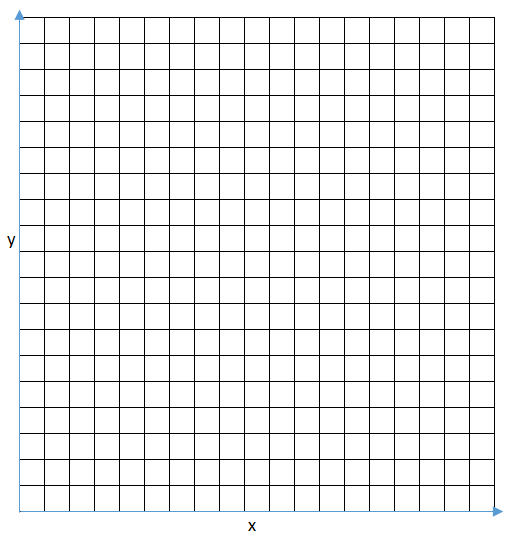
\includegraphics[width=0.5\textwidth]{grid1.png}
\caption{Cartesian grid representation of survey area. Origin (0,0) is in bottom left corner}
  \label{fig:grid}
\end{figure}

The robot will move in increments of one grid square, with a brief pause between increments (even in automatic modes). This ensures that sensor readings can be taken in each grid square without ambiguity. In the case where a significant feature (i.e. a faultline) is narrow and falls between robot halt points, the feature will be mapped to the nearest applicable grid square.

\subsection{Navigation}\label{navoverview}
In move-to-point mode, the path between the start and end grid squares is calculated using an A* search method with a Manhattan heuristic (performed by the Navigation controller--see Section \ref{navigation}) \cite{jones}. The sequence of moves is then passed to the Movement Controller (see Section \ref{movement}) which is responsible for making the appropriate RMI calls to the robot's actuators and correcting its course based on feedback from the Sensor Controller (see Section \ref{sensors}).

Fully autonomous mode is merely an extension of move-to-point mode in that a series of waypoints are defined based on the expected size of the survey area and any known obstacles. The navigation tree is rebuilt after each navigation step, or when an unexpected obstacle is encountered. The survey area is traversed in a spiral pattern (see Figure \ref{fig:spiral}) in an attempt to minimise the number of turns required to traverse the entire area due to the angular accuracy problem mentioned in Section \ref{hardware}.

\begin{figure}[!htb]
\centering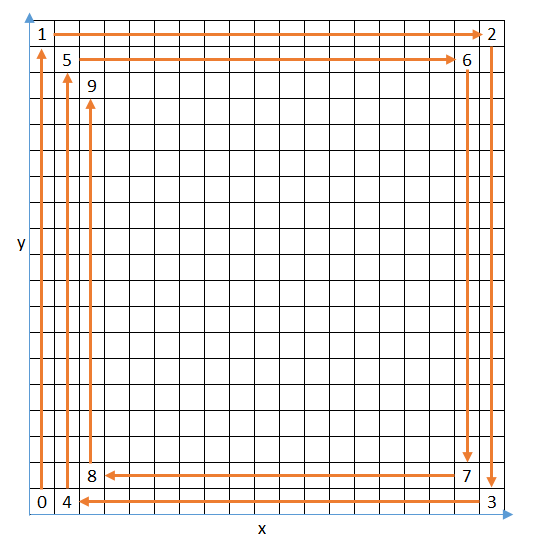
\includegraphics[width=0.5\textwidth]{grid2.png}
\caption{First nine points of autonomous navigation pattern. Point zero is the assumed start point}
  \label{fig:spiral}
\end{figure}

\FloatBarrier
\section{System Architecture and Components Design}

\subsection{Architectural Description}\label{architecture}
The Prospector SFM system consists of six major sections: 
\begin{itemize}
\item Graphical user interface (Operations GUI)
\item Data (file) input/output
\item Mapping system
\item Movement system
\item Sensor system
\item Remote connection system
\end{itemize}
Each of these systems is encapsulated in a Java package under the top-level Prospector package, as represented in Figure \ref{fig:architecture}, in order to enforce an appropriate level of separation of concerns. Communication between top-level classes in different packages is via the Observer pattern \cite{buschmann}; each package contains interfaces which can be implemented by other classes in order to receive asynchronous callbacks based on important events. The interfaces provided in each package are also shown in Figure \ref{fig:architecture}. The details of these interfaces and their implementing classes is discussed in Section \ref{detailed}.

A key architectural decision was to execute all control logic off-board (i.e. on the operator workstation rather than on the EV3 hardware platform) and directly invoke sensor readings and actuator motion via the LeJOS-provided RMI interfaces. Alternatives to this architectural choice and the rationale for making this decision are discussed in Sections \ref{alternative} and \ref{rationale}, respectively.

\begin{figure}[!htb]
\centering\includegraphics[width=\textwidth]{architecture.png}
\caption{Prospector SFM software system architecture overview}
  \label{fig:architecture}
\end{figure}

\subsection{Component Decomposition Description}
Each of the major components listen in Section \ref{architecture} communicates with one or more other major components by implementing a listener interface from the appropriate package. Each major component maintains an internal list of listeners which have registered to receive callbacks for a particular event type, and components register to receive events from each other via public registration and methods. For example, the Movement Controller instance is registered as a listener to the Connection Controller instance and subsequently receives a callback from that instance when a connection with the remote EV3 robot has been established (or when a connection attempt has failed). For simplicity and to enforce separation of concerns, each listener interface contains only one abstract method.

In general, components register as listeners with each other in the Prospector class, which is the main Java class for the system, prior to display of the GUI (i.e. the JavaFX \textit{launch} method). As only one of each major class is required for operation of the system, each of these classes exists as a single static instance declared in the Prospector class and instantiated in either the static \textit{main} method or the \textit{launch} method.

Because the GUI framework of choice was JavaFX (see Section \ref{GUI} for rationale), the Prospector main class extends the JavaFX Application class, which in turn invokes the overridden \textit{launch} method in which GUI components are instantiated and displayed. 

Figure \ref{fig:observers} shows the channels of communication between major components via the Observer pattern. For details of the interfaces themselves, see Section \ref{detailed}. UML diagrams can be found in Section \ref{uml}.

\begin{figure}[!htb]
\includegraphics[width=\textwidth]{observers.png}
\caption{Communication between components via listener interfaces}
  \label{fig:observers}
\end{figure}

\subsection{Detailed Components Design Description}\label{detailed}

The functionality of each subsystem component is discussed below, along with an overview of the public methods for each top-level controller class, and the interfaces implemented and provided by each. Also, the SRS requirements covered by each component are referenced.

\FloatBarrier
\subsubsection{C001 - Main Window Controller}
\begin{description}
\item [{Purpose:}] URC001-009, URE001-004
\item [{Function: }] The Main Window Controller is the controller part of the JavaFX GUI implementation (see Section \ref{GUI}), and converts user input (button presses, text field inputs) to a form which can be translated to commands for other system components. 
\item[{Subordinates: }] None
\item[{Dependencies: }] C002, C003, C004, C005
\item[{Interfaces: }] The Main Window controller provides no interfaces to other components, but holds a direct reference to both the Movement and Connection controllers in order to invoke robot movement commands and connection attempts, respectively. Further details of the GUI functionality is provided in Section \ref{GUI}.
\item[{Data: }] None.
\end{description}

\FloatBarrier
\subsubsection{C002 - Connection Controller}
\begin{description}
\item [{Purpose:}] FRC005, FRC006, FRC007
\item [{Function: }] The Connection Controller does is responsible for establishing a connection to the remote robot, and creating references to each of the required hardware components so that they can be controlled and monitored via RMI. The Connection Controller's public methods are listed in Table \ref{table:connectioncontroller}.

\begin{table}
\begin{tabular}{ | p{0.27\textwidth} | p{0.25\textwidth} |p{0.25\textwidth}|p{0.28\textwidth}|}
\hline
\textbf{Method name} & \textbf{Return type} & \textbf{Parameters} & \textbf{Description} \\
\hline
setAddress & void & String & Sets the IP address for the remote robot connection \\
\hline
connect & void & void & Initiates a connection attempt to the remote robot \\
\hline
getConnected & boolean & void & Returns true if a connection has been established to the robot, false otherwise \\
\hline
closeAll & void & void & Shuts down all remote hardware ports \\
\hline
addConnectionListener & void & ConnectionListener & Adds a listener for connection events \\
\hline
getMotorA & RMIRegulatedMotor & void & Returns a reference to the robot's "A" motor, which can be used for RMI calls \\
\hline
getMotorB & RMIRegulatedMotor & void & Returns a reference to the robot's "B" motor, which can be used for RMI calls \\
\hline
getMotorD & RMIRegulatedMotor & void & Returns a reference to the robot's "D" motor, which can be used for RMI calls \\
\hline
getUltSample & RMISampleProvider & void & Returns a reference to the robot's ultrasonic sensor, which can be used for RMI calls \\
\hline
getGyroSample & RMISampleProvider & void & Returns a reference to the robot's gyroscopic sensor, which can be used for RMI calls \\
\hline
getColourSample & RMISampleProvider & void & Returns a reference to the robot's colour sensor, which can be used for RMI calls \\
\hline
\end{tabular}
\caption{ConnectionController public methods}
\label{table:connectioncontroller}
\end{table}

\item[{Subordinates: }] None
\item[{Dependencies: }] None

\item[{Interfaces: }] The Connection Controller provides the ConnectionListener interface in order to allow other components to receive notification when a connection attempt has succeeded or failed. The methods provided by this interface are shown in Table \ref{table:connectionlistener}.

\begin{table}
\begin{tabular}{ | p{0.3\textwidth} | p{0.1\textwidth} |p{0.25\textwidth}|p{0.35\textwidth}|}
\hline
\textbf{Method name} & \textbf{Return type} & \textbf{Parameters} & \textbf{Description} \\
\hline
connectionStateChanged & void & boolean & Indicates success or failure of a connection attempt \\
\hline
\end{tabular}
\caption{ConnectionListener public methods}
\label{table:connectionlistener}
\end{table}

\item[{Data: }] The connection controller stores a string representing the IP address to use in order to connect to the robot, and references to the individual hardware components' RMI interfaces.
\end{description}
\FloatBarrier
\subsubsection{C003 - Movement Controller}\label{movement}
\begin{description}
\item [{Purpose \& Function:}] The Movement Controller is responsible for controlling the movement of the robot via remote method invocation based on user input. The implementation of the Movement Controller is split into three modes: Manual Control Mode, Move-to-Point Mode and Fully Autonomous Mode. The details of these are broken down below, and the Movement Controller's public methods are listed in Table \ref{table:movementcontroller}.
\paragraph{(1) Manual Mode}
\begin{description}
\item [{Purpose:}] FRC005
\item [{Function: }] The Manual Control Mode allows the user to manually control the movement of the robot from GUI. 
\end{description}
\paragraph{(2) Fully Autonomous Mode}
\begin{description}
\item [{Purpose:}] FRC006, FRC007
\item [{Function: }] The Fully Autonomous Mode allows robot to find a path from current location to destination provided by operator from GUI. It also allows robot to survey an area automatically.
\end{description}
\paragraph{(3) Move-to-Point Mode}
\begin{description}
\item [{Purpose:}] FRC001, FRC002, FRC003, FRC004
\item [{Function: }] In Move-to-Point mode, the robot will move to the specified point, avoiding obstacles and no-go-zones. 
\end{description}
\end{description}

\tablefirsthead{%
\hline
\multicolumn{1}{|l}{\textbf{Method name}} &
\multicolumn{1}{|l}{\textbf{Return type}} &
\multicolumn{1}{|l}{\textbf{Parameters}} &
\multicolumn{1}{|l|}{\textbf{Description}}\\
\hline
}
\tablehead{%
\hline
\multicolumn{4}{|l|}{\small\sl continued from previous page}\\
\hline
\multicolumn{1}{|l}{\textbf{Method name}} &
\multicolumn{1}{|l}{\textbf{Return type}} &
\multicolumn{1}{|l}{\textbf{Parameters}} &
\multicolumn{1}{|l|}{\textbf{Description}}\\
\hline
}
\tabletail{%
\hline
\multicolumn{4}{|l|}{\small\sl continued on next page}\\
\hline
}
\tablelasttail{\hline}
\bottomcaption{MovementController public methods}
\label{table:movementcontroller}
\begin{supertabular}
{ | p{0.27\textwidth} | p{0.25\textwidth} |p{0.25\textwidth}|p{0.28\textwidth}|}
\hline
setMoveMode & void & MoveMode & Sets the move mode of Movement Controller \\
\hline
startSurvey & void & Integer[] & Starts survey based on current mode. Survey a path from current position to a destination in Move-to-Point mode. Survey whole area in Fully Autonomous mode. \\
\hline
connect & void & Navigation & Connects MovementController class to Navigation class \\
\hline
connect & void & MappingController & Connects MovementController class to MappingController class \\
\hline
forwardCommand & void & void & Processes a manual forward command \\
\hline
backwardCommand & void & void & Processes a manual backward command \\
\hline
leftCommand & void & void & Processes a manual left turn command \\
\hline
rightCommand & void & void & Processes a manual right turn command \\
\hline
stop & void & void & Stops the robot from moving\\
\hline
addLocationListener & void & LocationListener & Adds a LocationListenter to the internally maintained list \\
\hline
setLocation & void & double, double, float & Sets the current location and broadcast location to every listener\\
\hline
startSurvey & void & integer[ ] & Initiates survey or movement to specified x, y destination, depending on mode \\
\hline
\end{supertabular}

\begin{description}
\item[{Subordinates: }] C003.1
\item[{Dependencies: }] C002, C004, C005
\item[{Interfaces: }] The Movement Controller provides the LocationListener interface in order to allow other components to receive notification when the robot move to a new position. The methods provided by this interface are shown in Table\ref{table:locationlistener}.

\begin{table}[!hpt]
\begin{tabular}{ | p{0.3\textwidth} | p{0.1\textwidth} |p{0.25\textwidth}|p{0.35\textwidth}|}
\hline
\textbf{Method name} & \textbf{Return type} & \textbf{Parameters} & \textbf{Description} \\
\hline
locationReceived & void & double, double, float, float & Indicates the location and direction of the robot \\
\hline
\end{tabular}
\caption{LocationListener public methods}
\label{table:locationlistener}
\end{table}

\item[{Data: }] The movement controller stores a integer representing the direction of robot(North, East, South, West). The movement controller stores an enum which named MoveMode representing the mode of movement (Manual, Move-to-Point or Fully Autonomous).
\end{description}

\FloatBarrier
\subsubsection{C003.1 - Navigation Controller}\label{navigation}
\begin{description}
\item [{Purpose:}] FRC004, FRC006, FRC007
\item [{Function: }] As a subordinate of the Movement Controller, the Navigation controller provides the path-finding functionality required to enable autonomous robot movement. Given a destination in (x,y) grid coordinates, it performs an A* search algorithm in order to find a path from its current location to the destination. When invoked from the Movement Controller, it returns a list of movements required to reach the destination. This controller's public methods are listed in Table \ref{table:navigation}.

\begin{table}
\begin{tabular}{ | p{0.27\textwidth} | p{0.25\textwidth} |p{0.25\textwidth}|p{0.28\textwidth}|}
\hline
\textbf{Method name} & \textbf{Return type} & \textbf{Parameters} & \textbf{Description} \\
\hline
run & List<Integer[ ]> & Integer[ ] & Given a destination in (x, y) coordinates, returns a list of waypoints in (x, y) coordinates based on A* algorithm \\
\hline
connect & void & MovementController & Sets a reference to the MovementController class \\
\hline
\end{tabular}
\caption{NavigationController public methods}
\label{table:navigation}
\end{table}

\item[{Subordinates: }] None
\item[{Dependencies: }] C003, C005
\item[{Interfaces: }] None.
\item[{Data: }] The navigation controller stores and updates the tree of movements required to reach the current target destination.
\end{description}

\FloatBarrier
\subsubsection{C004 - Sensor Controller}\label{sensors}
\begin{description}
\item [{Purpose \& function:}] The Sensor Controller is responsible for controlling the sensors of the robot. The implementation of the Sensor Controller is made up of Color Sensor Controller, Gyro Sensor Controller and Ultrasonic Sensor Controller. Purpose and function for each part is as follow. The Sensor Controller's public methods are listed in Table \ref{table:sensorcontroller}
\end{description}
\tablefirsthead{%
\hline
\multicolumn{1}{|l}{\textbf{Method name}} &
\multicolumn{1}{|l}{\textbf{Return type}} &
\multicolumn{1}{|l}{\textbf{Parameters}} &
\multicolumn{1}{|l|}{\textbf{Description}}\\
\hline
}
\tablehead{%
\hline
\multicolumn{4}{|l|}{\small\sl continued from previous page}\\
\hline
\multicolumn{1}{|l}{\textbf{Method name}} &
\multicolumn{1}{|l}{\textbf{Return type}} &
\multicolumn{1}{|l}{\textbf{Parameters}} &
\multicolumn{1}{|l|}{\textbf{Description}}\\
\hline
}
\tabletail{%
\hline
\multicolumn{4}{|l|}{\small\sl continued on next page}\\
\hline
}
\tablelasttail{\hline}
\bottomcaption{SensorController public methods}
\label{table:sensorcontroller}
\begin{supertabular}
{ | p{0.27\textwidth} | p{0.25\textwidth} |p{0.25\textwidth}|p{0.28\textwidth}|}
\hline
addColourListener & void & ColourListener & Adds a ColourListener to the list, it can detect any color changing from color sensor  \\
\hline
addDistanceListener & void & DistanceListener & Adds a DistanceListener to the list, it can receive distance change from movement Class \\
\hline
addAngleListener & void & GyroListener & Adds a AngleListener to the list, it can detect any angle changing form angle sensor\\
\hline
broadcastColour ToListeners & void & void & Informs all color listeners of the current color reading, and it can be called any time \\
\hline
broadcastDistance ToListeners & void & void & Informs all distance listeners of the current distance reading, and it can be called any time \\
\hline
broadcastAngle ToListeners & void & void & Informs all angel listeners of the current angel reading, and it can be called any time\\
\hline
start & void & void & Starts thread of sensor to detect distance, gyro and colour  \\
\hline
getDistance & float & void & Gets data of distance from ultrasonic sensor \\
\hline
startDistanceThread & void & void & Starts a thread to keep reading distance from ultrasonic sensor and broadcast the data to every listeners \\
\hline
startGyroThread & void & void & Starts a thread to keep reading angle from gyro sensor and broadcast the data to every listeners \\
\hline
startColourThread & void & void & Starts a thread to keep reading colourid from colour sensor and broadcast the data to every listeners \\
\hline
shutdown & void & void & Closes threads of distance, gryo and colour\\
\hline
\end{supertabular}

\begin{description}
\item[{Subordinates: }] None
\item[{Dependencies: }] None
\item[{Interfaces: }] The Sensor Controller provides the ColourListener, GyroListener and DistanceListener interfaces. The ColourListener allows other components to receive the colorID detected by the colour sensor. The GyroListener allows other components to receive the rotation angle detected by the gyro sensor. The DistanceListener allows other components to receive the distance between an obstacle and robot detected by the Ultrasonic sensor. The methods provided by these interfaces are shown in Table\ref{table:sensorlistener}.

\begin{table}
\begin{tabular}{ | p{0.3\textwidth} | p{0.1\textwidth} |p{0.25\textwidth}|p{0.35\textwidth}|}
\hline
\textbf{Method name} & \textbf{Return type} & \textbf{Parameters} & \textbf{Description} \\
\hline
colourDetected & void & float & Indicates the color detected by the color sensor \\
\hline
distanceReceived & void & float & Indicates the distance detected by the ultrasonic sensor \\
\hline
angleReceived & void & float & Indicates the angle detected by the gyro sensor \\
\hline
\end{tabular}
\caption{SensorListener public methods}
\label{table:sensorlistener}
\end{table}

\item[{Data: }] The sensor controller stores a float representing the color, a float representing the distance and a float representing the rotation angle degree.
\end{description}

\paragraph{(1) Color Sensor Controller}
\begin{description}
\item [{Purpose:}] FRC002, FRC004, FRC0015, FRC0016
\item [{Function: }] The color sensor will detects the colorID of current position of robot and broadcasts it to other components.
\end{description}

\paragraph{(2) Gyro Sensor Controller}
\begin{description}
\item [{Purpose:}] FRC001
\item [{Function: }] The Gyro sensor will detects the rotation angle of robot and broadcasts it to other components.
\end{description}

\paragraph{(3) Ultrasonic Sensor Controller}
\begin{description}
\item [{Purpose:}] FRC003
\item [{Function: }] The Ultrasonic sensor will detects the distance around current position of a robot and broadcasts it to other components.
\end{description}


\FloatBarrier
\subsubsection{C005 - Mapping Controller}
\begin{description}
\item [{Purpose:}] URC005, FRC008, FRC009
\item [{Function: }] The Mapping Controller maintains the internal map data model representing the surveyed area, and determines the position of mapped environmental features by synthesising the input from the sensors (via the Sensor Controller) with the robot's current position (via the Movement Controller). This controller's public methods are listed in Table \ref{table:mappingcontroller}.

\begin{table}
\begin{tabular}{ | p{0.2\textwidth} | p{0.2\textwidth} |p{0.2\textwidth}|p{0.4\textwidth}|}
\hline
\textbf{Method name} & \textbf{Return type} & \textbf{Parameters} & \textbf{Description} \\
\hline
addMapListener & void & MapListener & Registers a listener for map data model updates \\
\hline
setMapMode & void & boolean & Turns the mapping functionality on or off.\\
\hline
getDataModel & MapDataModel & void & Returns the current version of the map data model representing the survey area \\
\hline
clearMap & void & void & Clears the map data model; marks all areas as unexplored \\
\hline
shutdown & void & void & Stops the scheduled dispatch of data model updates to listeners \\
\hline
\end{tabular}
\caption{MappingController public methods}
\label{table:mappingcontroller}
\end{table}

\item[{Subordinates: }] None
\item[{Dependencies: }] C003, C004

\item[{Interfaces: }]  The Mapping Controller implements the LocationListener, ColourListener and DistanceListener interfaces. The Mapping Controller provides the MapListener interface in order to allow other components to receive notification when the internal map data model has been updated. The methods provided by this interface are shown in Table \ref{table:maplistener}.

\begin{table}
\begin{tabular}{ | p{0.3\textwidth} | p{0.1\textwidth} |p{0.25\textwidth}|p{0.35\textwidth}|}
\hline
\textbf{Method name} & \textbf{Return type} & \textbf{Parameters} & \textbf{Description} \\
\hline
mapDataReceived & void & MapDataModel & Passes the current version of the map data model \\
\hline
\end{tabular}
\caption{MapListener public methods}
\label{table:maplistener}
\end{table}

\item[{Data: }] The Mapping Controller stores the current data model of the survey area in a MapDataModel object (see section \ref{Data}).

\end{description}
\FloatBarrier
\subsubsection{C006 - Data Controller}
\begin{description}
\item [{Purpose:}] FRC011, FRC012, FRC013
\item [{Function: }] The Data Controller handles the import and export of map data files, both in response to user demand and on a periodic basis for data backup and recovery. This controller's public methods are listed in Table \ref{table:datacontroller}.

\begin{table}[h!]
\begin{tabular}{ | p{0.2\textwidth} | p{0.2\textwidth} |p{0.2\textwidth}|p{0.4\textwidth}|}
\hline
\textbf{Method name} & \textbf{Return type} & \textbf{Parameters} & \textbf{Description} \\
\hline
writeFileOut & void & MapDataModel, File & Writes the map data model to an XML file \\
\hline
readFileIn & MapDataModel & URL & Reads a file specified by the URL and returns a MapDataModel object \\
\hline
\end{tabular}
\caption{DataController public methods}
\label{table:datacontroller}
\end{table}

\item[{Subordinates: }] None
\item[{Dependencies: }] C005

\item[{Interfaces: }] The Data Controller implements the MapListener interface in order to receive map data model updates for periodic backup.

\item[{Data: }] None.

\end{description}

\FloatBarrier
\subsection{Architectural Alternatives}\label{alternative}
A major architectural decision made early in the design process was to keep all logic and control modules off-board, that is, executed on the operator's workstation. An alternative would have been to compile some or all of the control logic into a LeJOS-executable JAR file to be run on the robot hardware itself, leaving only GUI and file input/output code to be run on the operator's workstation. Communication between the workstation and the robot would have been via a custom-developed communication protocol built on Java sockets. This approach would have had the following advantages:
\begin{itemize}
\item Ability to continue to execute on-board logic functions such as survey area exploration and updates to internal data model even in the event of transient loss of communication to operator workstation
\item Ability to execute emergency evasive action/stop even in the event of loss of communication to operator workstation
\end{itemize}
Disadvantages of such an approach include:
\begin{itemize}
\item Requirement to design and implement a custom communications protocol, representing an additional possible failure mode during operation
\item Requirement to design and implement two separate but related Java projects: one for the LeJOS platform (on-board) and one for the operator workstation (off-board)
\end{itemize}

\subsection{Design Rationale}\label{rationale}
The decision to implement each major functional area of the system as a separate major class in its own package is consistent with the principle of separation of concerns, the advantages of which have been well-established in the literature \cite{hursch}. The use of the observer pattern with asynchronous callbacks and (where appropriate) scheduled dispatch of data to registered listeners is also consistent with best practices in Java programming \cite{buschmann}. This approach allows for unit testing of each component, as well as progressive integration testing (provided interconnected components can be mocked where necessary for testing).

The architectural alternative discussed in Section \ref{alternative} was discarded due to its added complexity. As well as this, the LeJOS platform already provides a low-level RMI mechanism which can be used for off-board control of motors, making the development of a custom communications protocol an unnecessary additional component. 

The major concession made in order to accommodate this design is the step-wise (rather than continuous) movement of the robot. This ensures that in the event of a loss of communication between the robot and workstation, the robot will not move further than one grid square before coming to a halt.

\section {Data Design}\label{Data}

\subsection{Data Model Description}
The Prospector SFM software system contains one major data structure used for passing  state information between the separate system components. This the MapDataModel class, which includes the robot position model. 

\subsection{Data Structures}

\subsubsection{MapDataModel}
The MapDataModel object represents the current state of the mapped survey area. It fundamentally consists a grid of squares of predefined size, with each grid square represented by a GridSquare data object. The map data model is initialize once when it receives its dimensions (width, height) via its constructor from configured parameters, and is subsequently maintained by the Mapping Controller. The data members of the MapDataModel class are listed below:

\begin{description}
\item{\textbf{GridSquare[ ][ ] mapGrid: }} A two-dimensional matrix of GridSquare objects of configurable size representing the survey area.
\item{\textbf{Integer[ ] robotPosition: }} An integer array of length 2 representing the robot's current cartesian coordinates at the time the MapDataModel object was updated.
\end{description}

The public methods of the MapDataModel object are listed in Table \ref{table:mapdatamodel}.


\begin{table}
\begin{tabular}{ | p{0.22\textwidth} | p{0.2\textwidth} |p{0.3\textwidth}|p{0.33\textwidth}|}
\hline
\textbf{Method name} & \textbf{Return type} & \textbf{Parameters} & \textbf{Description} \\
\hline
getWidth & Integer & void & Returns the width of the map data model grid \\
\hline
getHeight & Integer & void & Returns the height of the map data model grid \\
\hline
validPoint & boolean & Integer[ ] & Returns true if the provided array represents a point within the defined grid \\
\hline
getGridSquare & GridSquare & Integer[ ] & Returns the grid square at the specified point \\
\hline
setGridSquare & void & Integer[ ], GridSquare & Sets the value of the grid square at the specified point \\
\hline
clear & void & void & Sets the entire map grid to UNKNOWN \\
\hline
setRobotPosition & void & Integer[ ] & Sets the current grid position of the robot \\
\hline
getRobotPosition & Integer[ ] & void & Returns the current grid position of the robot \\
\hline
\end{tabular}
\caption{MapDataModel public methods}
\label{table:mapdatamodel}
\end{table}

\subsubsection{GridSquare}
The GridSquare class represents a single square of the map data model grid. It consists of type designation in the form of a GridSquareEnum member and an Integer member representing a property of the GridSquare instance. This property is used in the case where a GridSquare object represents a fault line, and is used to store the color value of that fault line. The data members of the GridSquare class are listed below:

\begin{description}
\item{\textbf{GridSquareEnum value: }} The type of grid square represented by this object.
\item{\textbf{Integer property: }} A numerical representation of a relevant property of this grid square.
\end{description}

The only public methods of the GridSquare class are the public accessors of its two private members.

\subsubsection{GridSquareEnum}
The GridSquareEnum class is an integer-backed enumeration representing the possible contents of a grid square. Its possible values and their meaning are shown in Table \ref{table:gridsquareenum}.

\begin{table}[h!]
\begin{tabular}{ | p{0.2\textwidth} | p{0.1\textwidth} |p{0.6\textwidth}|}
\hline
\textbf{Name} & \textbf{Value} & \textbf{Description} \\
\hline
UNKNOWN & 0 & Unexplored area \\
\hline
BLANK & 1 & Explored and empty \\
\hline
FAULTLINE & 2 & Fault line \\
\hline
OBSTACLE & 3 & Three-dimensional obstacle \\
\hline
BOUNDARY & 4 & Survey area boundary \\
\hline
NGZ & 5 & Defined No-Go Zone \\
\hline
EXTRACTION & 6 & Robot extraction container area \\
\hline
ROBOT & 7 & Robot position at time of data model update \\
\hline
\end{tabular}
\caption{GridSquareEnum values}
\label{table:gridsquareenum}
\end{table}

\FloatBarrier
\section{Design Details}
\subsection{Class Diagrams}\label{uml}
The Prospector Sea Floor Mapping System divided into six parts (packages), and the UML diagram of their relationships is shown in Figure \ref{fig:Total}.
 \begin{figure}[!htb]
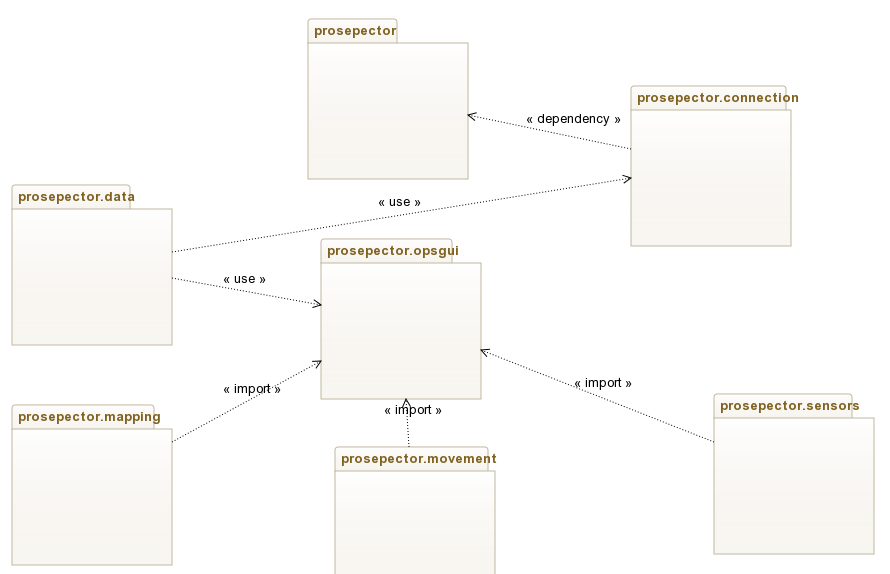
\includegraphics[width=\textwidth]{Total.png}
\caption{The UML diagram of the Prospector Sea Floor Mapping System }
  \label{fig:Total}
\end{figure}
In addition, more specific UML diagrams of each part are provided in Figures \ref{fig:SensorController} - \ref{fig:connection}.
\subsubsection{prospector.sensor} The UML diagram of sensor control system shown in Figure \ref{fig:SensorController}.
 \begin{figure}[!htb]
\centering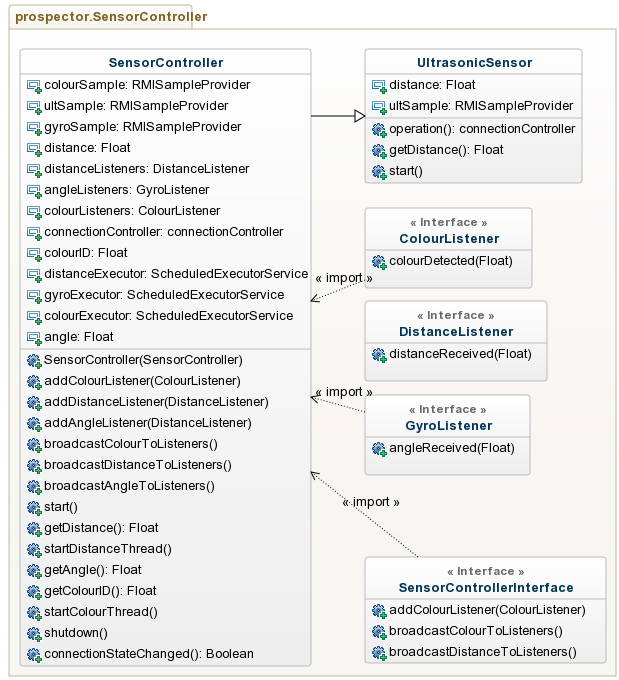
\includegraphics[width=0.7\textwidth]{SensorController.png}
\caption{The UML diagram of sensor controller }
  \label{fig:SensorController}
\end{figure}

\subsubsection{prospector.mapping}
The UML diagram of mapping system shown in Figure \ref{fig:mapping}.

\begin{figure}[!htb]
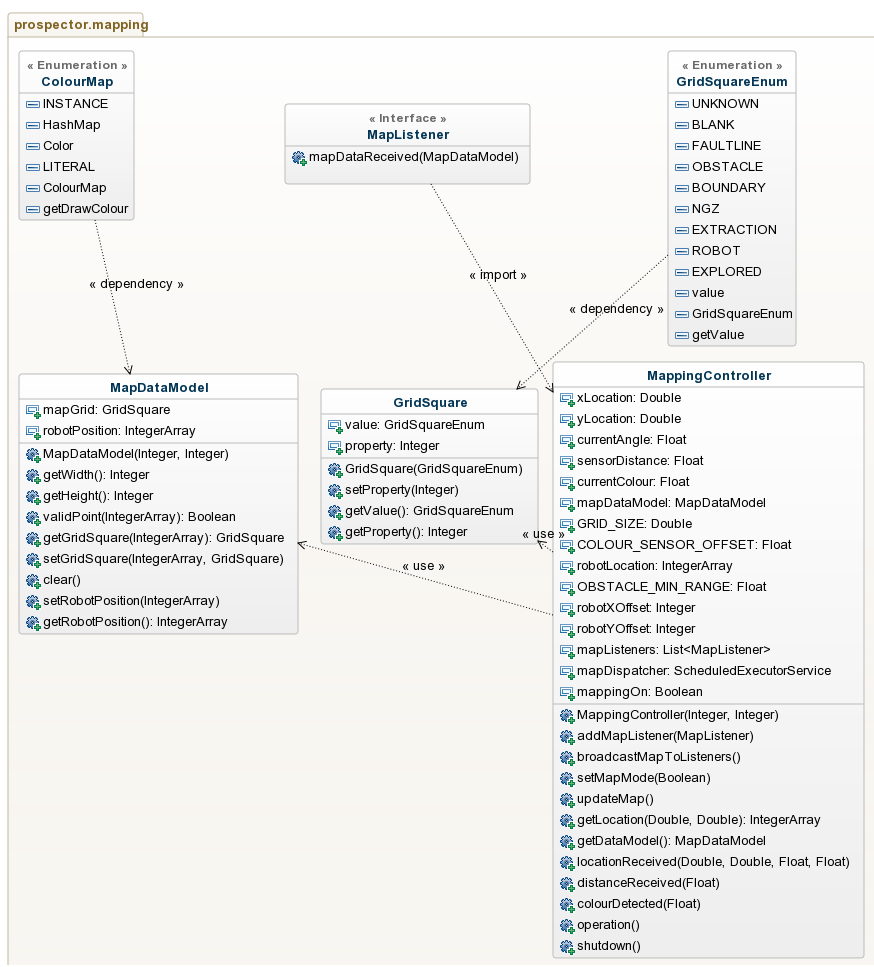
\includegraphics[width=\textwidth]{mapping.png}
\caption{The UML diagram of mapping }
  \label{fig:mapping}
\end{figure}

\subsubsection{prospector.opsgui}
The UML diagram of GUI shown in Figure \ref{fig:opsgui}.

\begin{figure}[!htb]
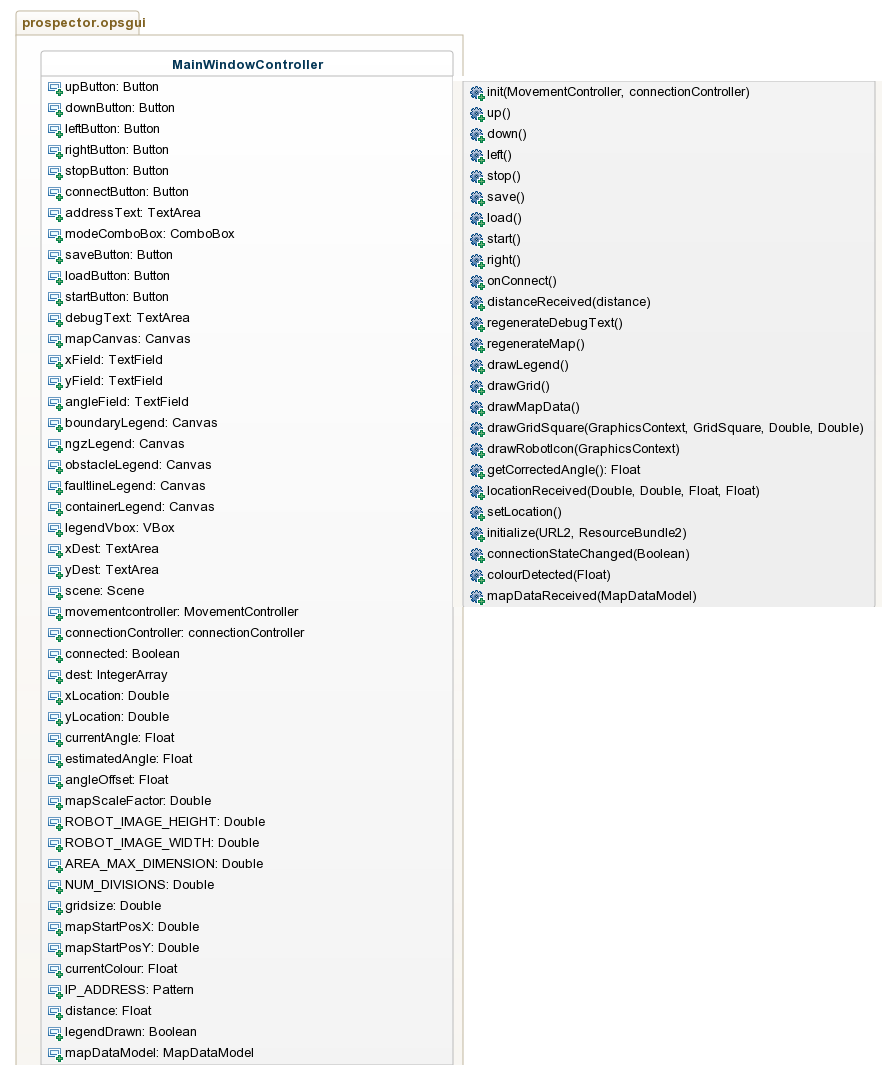
\includegraphics[width=\textwidth]{opsgui.png}
\caption{The UML diagram of GUI}
  \label{fig:opsgui}
\end{figure}

\subsubsection{prospector.movement}
The UML diagram of movement system shown in Figure \ref{fig:movement}.

\begin{figure}[!htb]
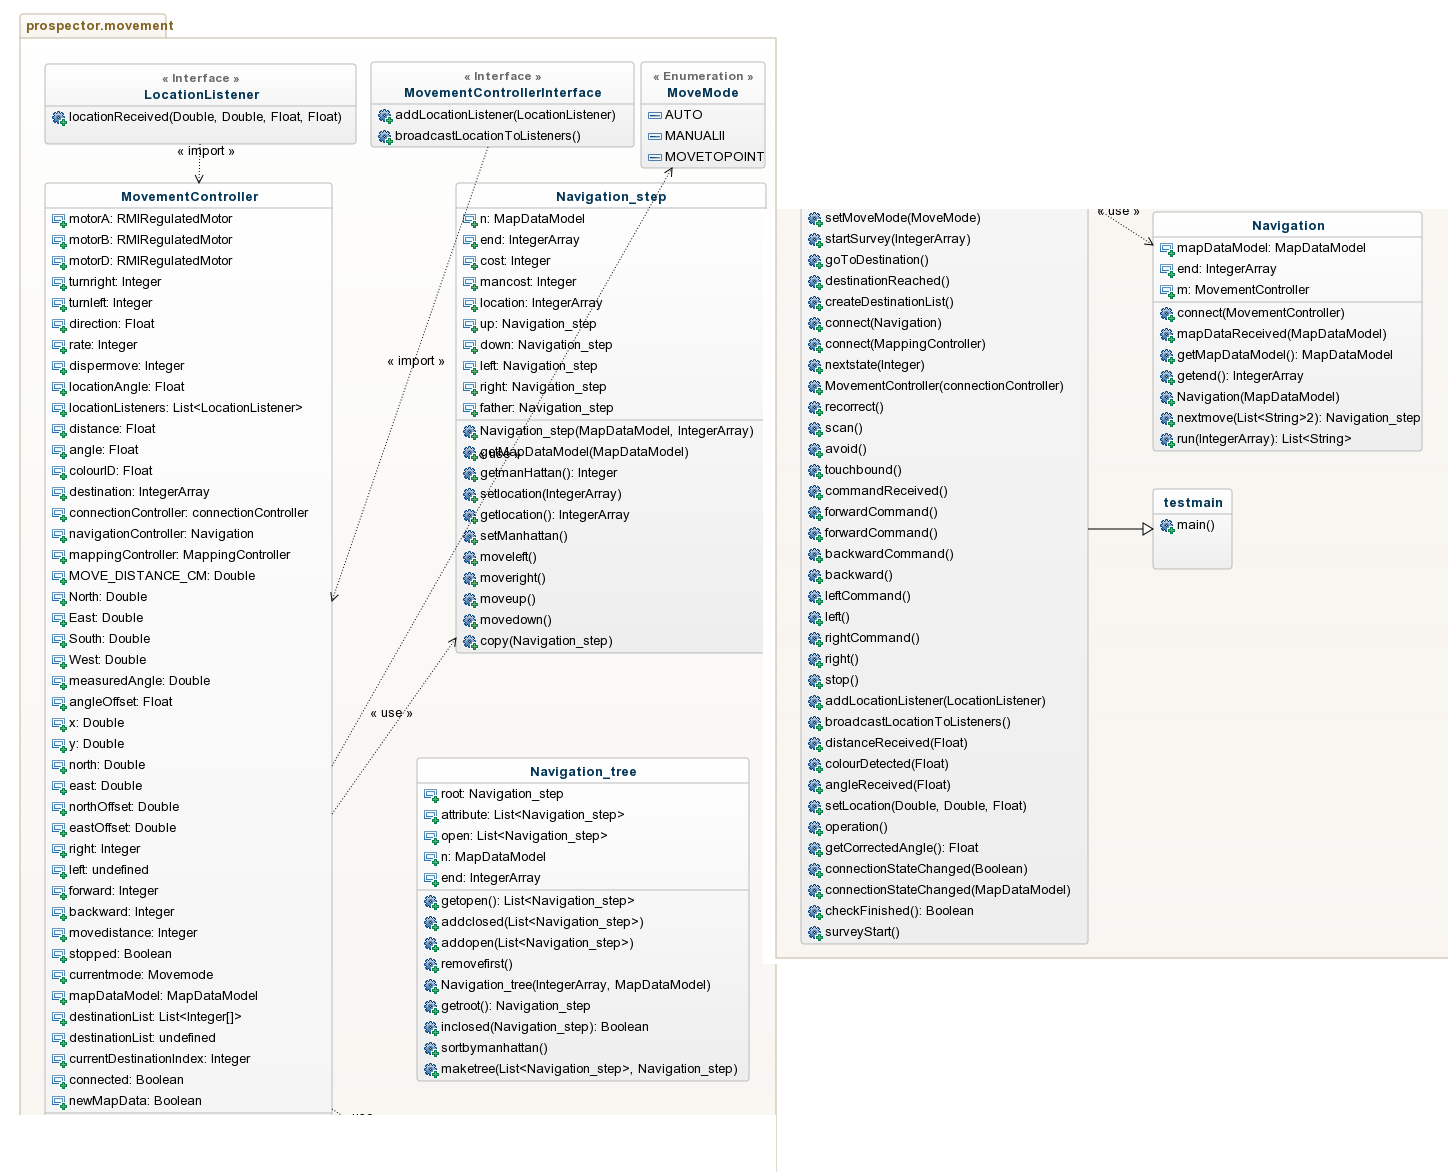
\includegraphics[width=\textwidth]{movement.png}
\caption{The UML diagram of movement}
  \label{fig:movement}
\end{figure}

\subsubsection{prospector.data}
The UML diagram of data collection system shown in Figure \ref{fig:data}.

\begin{figure}[!htb]
\centering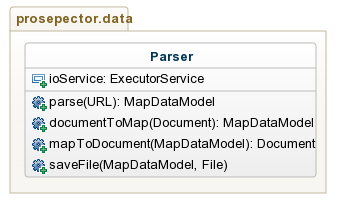
\includegraphics[width=0.5\textwidth]{data.png}
\caption{The UML diagram of data collection}
  \label{fig:data}
\end{figure}
\subsubsection{prospector.connection}
The UML diagram of connection system shown in Figure \ref{fig:connection}.

\begin{figure}[!htb]
\centering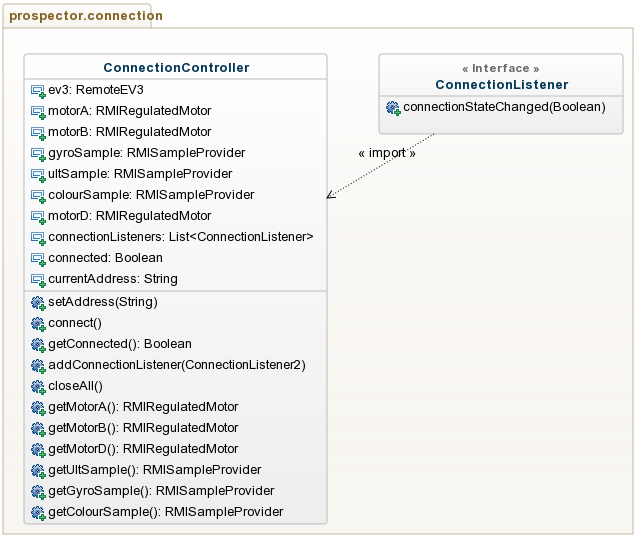
\includegraphics[width=0.5\textwidth]{connection.png}
\caption{The UML diagram of connection}
  \label{fig:connection}
\end{figure}

\FloatBarrier
\subsection{State diagrams}
The state diagram for the Navigation Controller in fully autonomous mode is shown in Figure \ref{fig:navstate}.

\begin{figure}[!htb]
\centering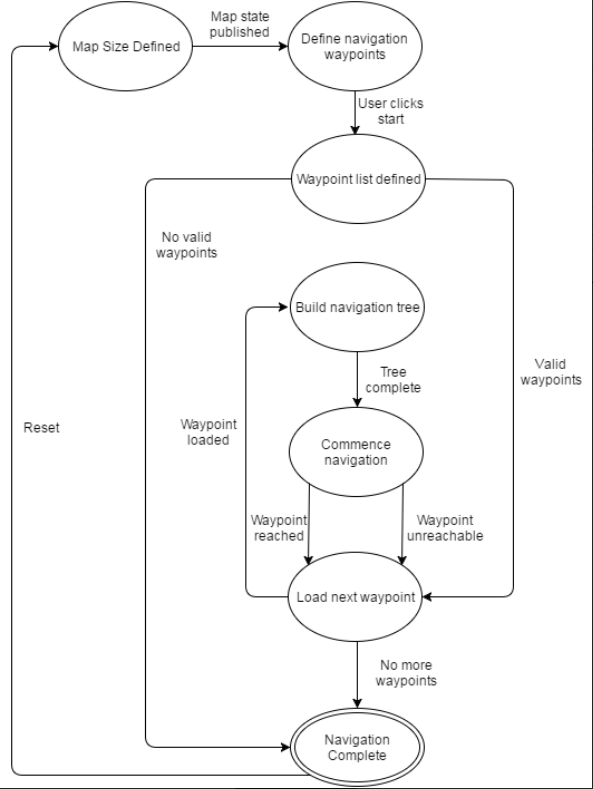
\includegraphics[width=0.6\textwidth]{navstate.png}
\caption{The state diagram of the Navigation controller in autonomous mode}
  \label{fig:navstate}
\end{figure}

\FloatBarrier
\section{Human Interface Design}\label{GUI}

\subsection{Overview of the User Interface}
The operation is on the right of the user interface. There are four buttons to control the movement of robot, and a stop button in the center of navigation buttons. The manual or automatic button determine the button is controlled manually or automatically. The "save map" stores the map which detected by sensor and "load map" button get a map input which means map is already given. The "set location" button sets the current location of robot manually. In addition, there is a text field showing the data of the current status of robot.

\subsection{Detailed Design of the User Interface}

\subsubsection {UI model}
The GUI for the Prospector SFM uses a Model-View-Controller (MVC) pattern in order to decouple control logic and internal data modeling from the view presented to the user. To this end, JavaFX was selected over Swing (the main alternative) as the UI framework of choice due to its ability to separate the declarative FXML layout (the view) from the linked controller class, which in turn is separate from the data model classes.

The user interface is shown in Figure \ref{fig:gui}. The various parts are identified below: 
\begin{enumerate}
\item  Five buttons are provided for users to control robot manually, including forward, backward, turn left, turn right and a stop button. When the user press a button, the robot will move according to the button.  
\item  A drop-down menu allows robot control mode selection (Manual, Move-to-Point or Fully Autonomous Mode). 
\item  At any time, the current map can be saved to an XML file, a map can be loaded, or the current map display can be cleared. 
\item  Users can set the current position and orientation of the robot.
\item  A panel displays real-time information from the robot.
\item  The user can define the robot's IP address and initiate the remote connection.
\item Updates to the map may be enabled or disabled
\item  A map legend is displayed next to the map.
\item  A real-time map shows survey progress.
\end{enumerate}

\begin{figure}[!htb]
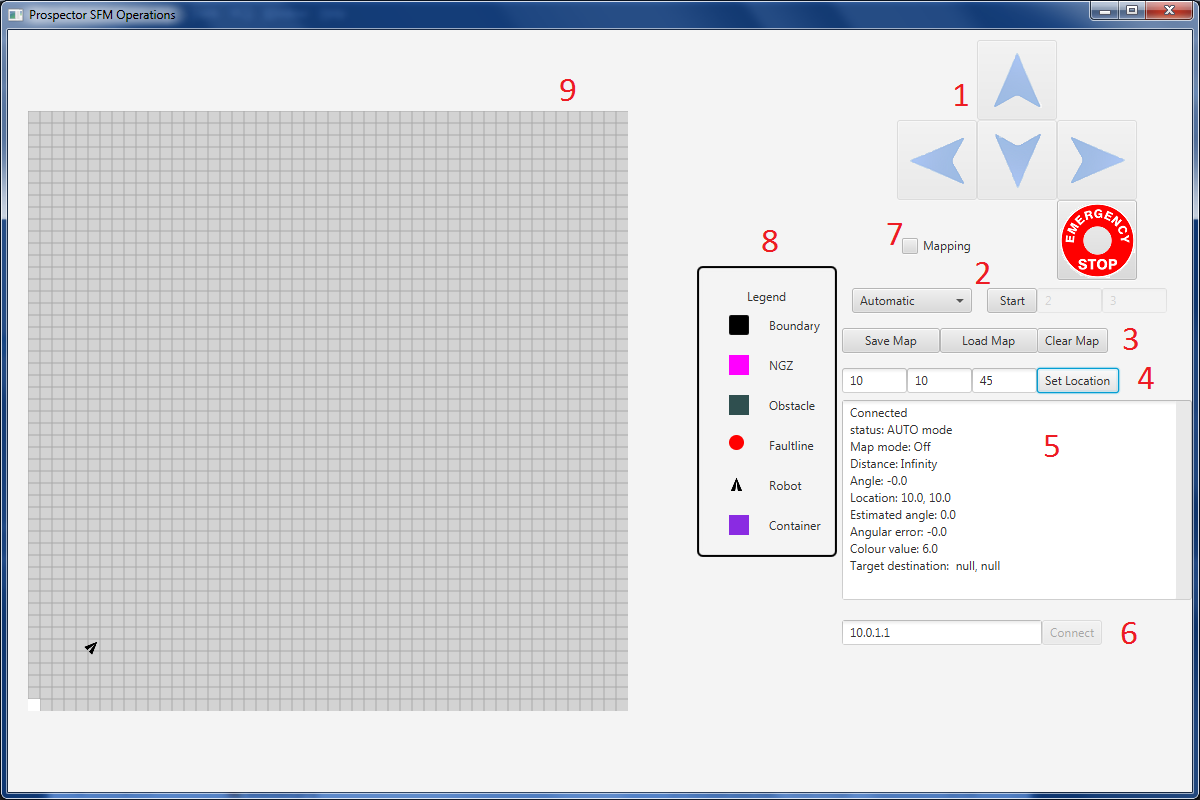
\includegraphics[width=\textwidth]{gui.png}
\caption{User interface}
  \label{fig:gui}
\end{figure}

\FloatBarrier
\section{Glossary}\label{glossary}

\begin{description}
\item [{GUI}] Graphical User Interface 
\item [{LeJOS}] The Lego Java Operating System 
\item [{RMI}] Remote Method Invocation 
\item [{SFM}] Sea Floor Mapping 
\item [{SRS}] Software Requirements Specification 
\item [{SDD}] Software Design Document 
\item[{MVC}] Model View Controller

\end{description}



\begin{thebibliography}{1}

\bibitem{buschmann} Buschmann, F, Henney, K and Schmidt, DC 2007. \textit{Pattern-Oriented Software Architecture: On Patterns and Pattern Languages}, Volume 5. Wiley and sons, West Sussex, England.

\bibitem{hursch} Hürsch WL and Lopes CV 1995. \textit{Separation of Concerns}. Northeastern University, Boston, USA. Technical report NU-CCS-95-03.

\bibitem{largemotor} LEGO Education, no date. \textit{EV3 Large Servo Motor}. Available online 1/10/2016 <https://education.lego.com/en-us/products/ev3-large-servo-motor/45502>

\bibitem{mediummotor} LEGO Education, no date. \textit{EV3 Medium Servo Motor}. Available online 1/10/2016 <https://shop.lego.com/en-US/EV3-Medium-Servo-Motor-45503>

\bibitem{ultrasonic} LEGO Education, no date. \textit{EV3 Ultrasonic Sensor}. Available online 1/10/2016 <https://shop.lego.com/en-US/EV3-Ultrasonic-Sensor-45504>

\bibitem{colour} LEGO Education, no date. \textit{EV3 Color Sensor}. Available online 1/10/2016 <https://education.lego.com/en-us/products/ev3-color-sensor/45506>

\bibitem{gyro} LEGO Education, no date. \textit{EV3 Gyro Sensor}. Available online 1/10/2016 <https://education.lego.com/en-us/products/ev3-gyro-sensor-/45505>

\bibitem{srs} Prospector Team 2016. \textit{Software Requirements Specification: Prospector Seafloor Mapping System}. Version 0.1 (Draft).

\bibitem{jones} 
Jones, MT 2008. \textit{Artificial Intelligence: A Systems Approach}. Jones and Bartlett Publishers, Sudbury, Massachusetts.
   
      

  \end{thebibliography}
\end{document}
